\documentclass[11pt, oneside]{article}   	% use "amsart" instead of "article" for AMSLaTeX format
\usepackage{geometry}                		% See geometry.pdf to learn the layout options. There are lots.
\geometry{letterpaper}                   		% ... or a4paper or a5paper or ... 
%\geometry{landscape}                		% Activate for rotated page geometry
\usepackage[parfill]{parskip}    		% Activate to begin paragraphs with an empty line rather than an indent
\usepackage{graphicx}				% Use pdf, png, jpg, or eps§ with pdflatex; use eps in DVI mode
								% TeX will automatically convert eps --> pdf in pdflatex		
\usepackage{amssymb}
\usepackage{amsmath}

% for color text:
%\usepackage{xcolor}
\usepackage[usenames,dvipsnames]{xcolor} 

% for hyperlinks
\usepackage{hyperref}

% for feynman slashes: 
\usepackage{mathtools}% http://ctan.org/pkg/mathtools
\newcommand{\fsl}[1]{\ensuremath{\mathrlap{\!\not{\phantom{#1}}}#1}}% \fsl{<symbol>}

%SetFonts

%\title{Neutrino - DM Scattering}
%\author{Kiara Carloni}
%\date{\today}							% Activate to display a given date or no date

\begin{document}
%\maketitle

{\Large Neutrino - DM Scattering} \\
Kiara Carloni \\
\today

The models and calculations covered here feature in the following reference works:
\begin{itemize}
\item \href{https://arxiv.org/pdf/1612.08472.pdf}{Constraining Dark Matter Neutrino Interaction with High Energy Neutrinos}, Dec. 2016
\item \href{https://arxiv.org/pdf/1703.00451.pdf}{Imaging Galactic Dark Matter with High-Energy Cosmic Neutrinos}, Mar. 2021
\item Dark Matter-Neutrino Scattering in the Galactic Centre with IceCube, Adam McMullen (Thesis, May 2021)
\end{itemize} 

% In addition, \href{https://arxiv.org/pdf/1706.09895.pdf}{High-energy Neutrino Attenuation in the Earth and its Associated Uncertainties}, Jan. 2019, is an important reference for the linear algebra approach to solving the cascade equation.

\newpage
\section{\large Kinematics: }x

Neutrino - DM scattering is analogous to Compton scattering ($\gamma + e^- \to \gamma + e^-$) if we treat the neutrino as massless.
We can therefore follow the derivation in Peskin+Schroeder. \\

From P+S (4.79), p.106, we get the formula for the differential cross-section for $2 \to\ n$ scattering with the final state phase space integral: 
\[ d\sigma = \frac{1}{2E_A 2E_B} \frac{1}{\left| k_A / E_A - k_B / E_B \right| } d\Pi_n \left|M\right|^2 \]

We will work in the lab frame (the dark matter rest frame). Here, we can write the initial and final four-momenta as: 

\begin{tabular}{p{6cm}c}
{\begin{align*}
    k_1 &= (E, 0, 0, E) \\
    k_2 &= (m_\chi, 0, 0, 0) \\
    p_1 &= (E', 0, -E' \sin\theta, E'\cos\theta) \\
    p_2 &= (\sqrt{m_\chi^2 +p'^2}, 0, p' \sin\psi, p'\cos\psi) 
\end{align*}}
&
 \raisebox{-3.4cm}{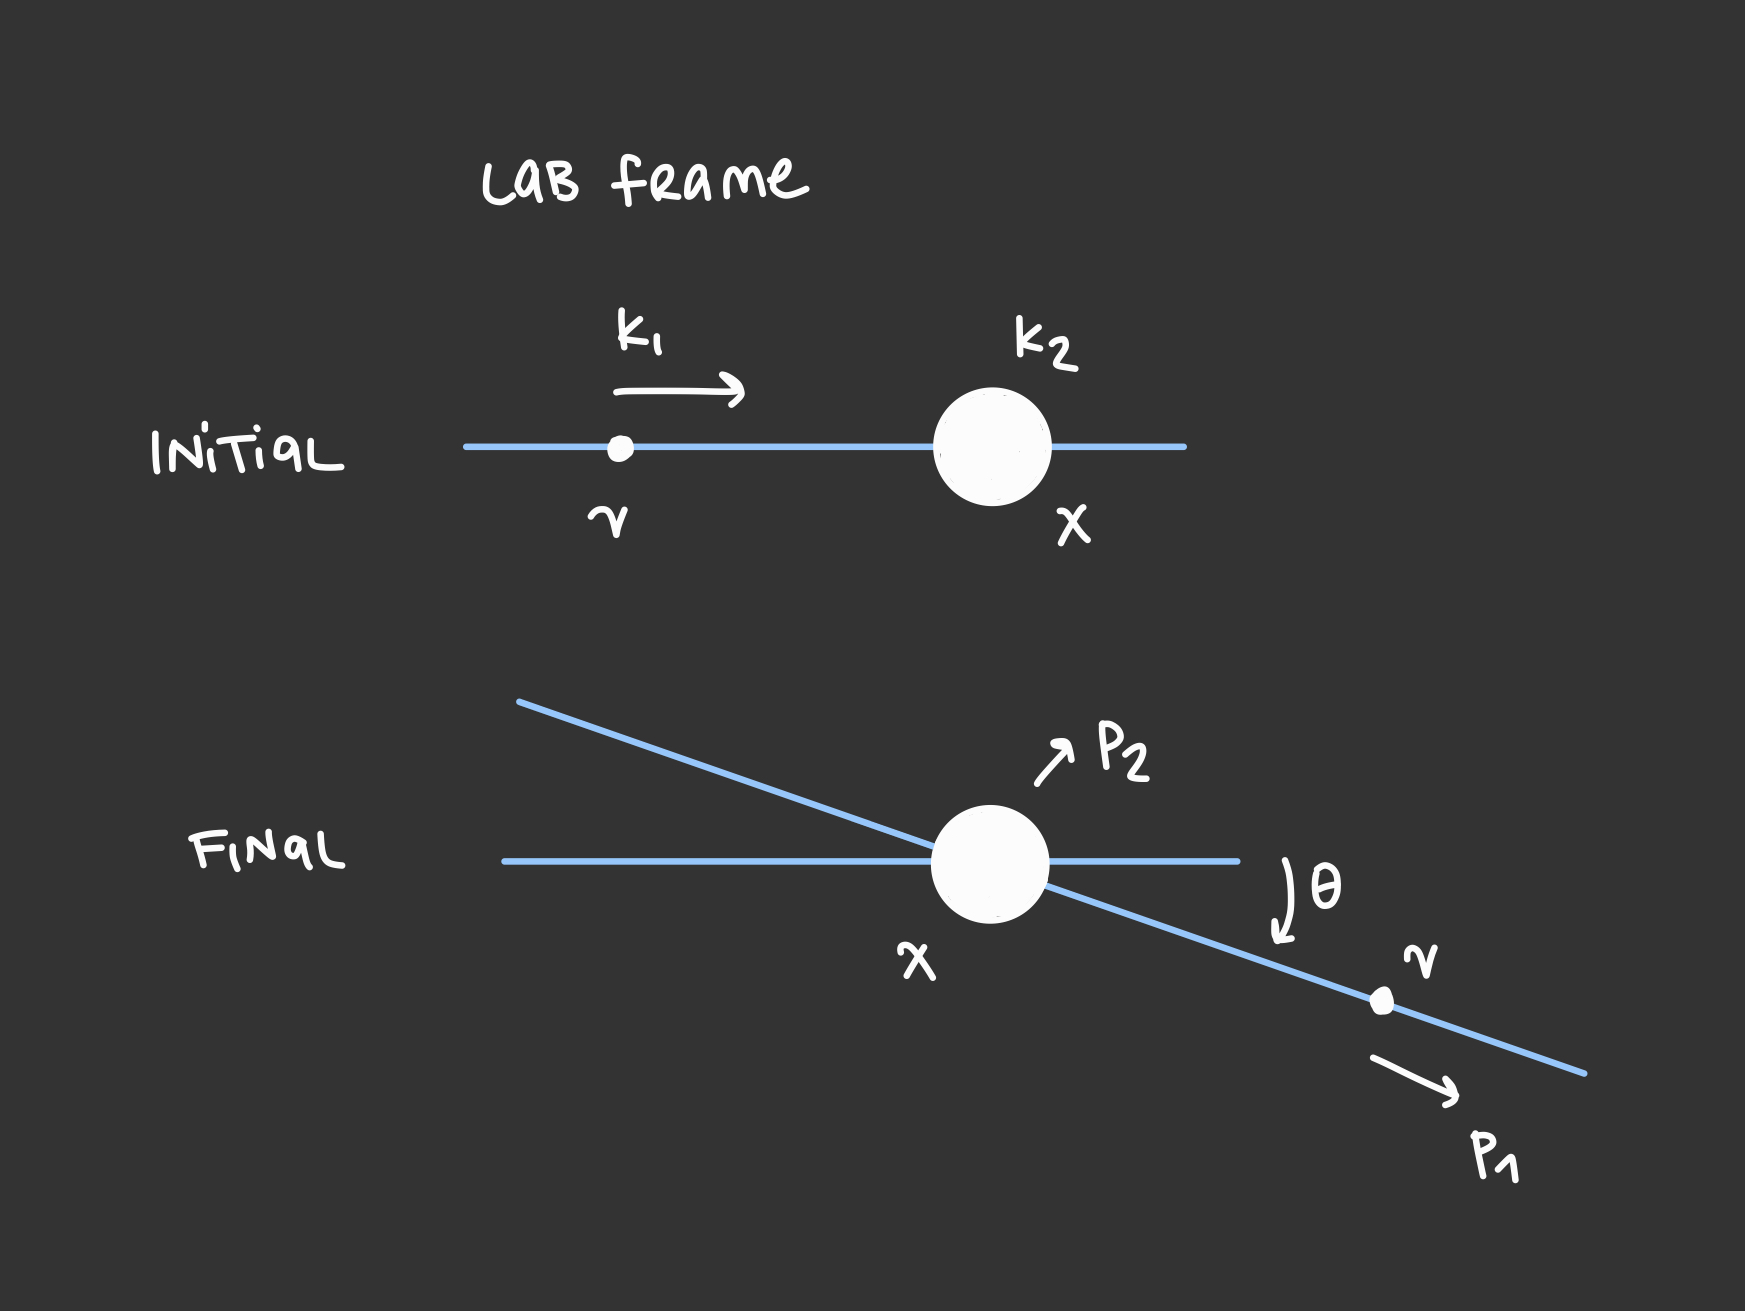
\includegraphics[width=5cm]{images/labframe_kinematics.jpeg}}
\end{tabular}

We can then solve for $E'$ as a function of $E, \theta$ by imposing four-momentum conservation, resulting in: 
%\tiny
%\begin{align*}
%0 &= -E' \sin\theta + p'\sin\psi \\
%E &=  E'\cos\theta + p'\cos\psi \\
%(E+m_\chi) &= E' + \sqrt{m_\chi^2 + p'^2} \\
%& \downarrow \\
%p'^2 & = E'^2 + E^2 - 2EE' \cos\theta \\
%       & = E'^2 + E^2 - 2EE' + 2(E-E')m_\chi \\
%& \downarrow
%\end{align*}
%\normalsize
\[ EE'(1-\cos\theta) = m\chi(E-E') \] 
\[ E' = \frac{E}{1 + E/m_\chi (1-\cos\theta)} \] 

\textbf{Note:} For fixed values of the initial energy $E$, there is a one-to-one relationship between the scattering angle $\theta$ and the final energy $E'$. 

By completing the phase-space integral (see P+S p.163) we find that
\begin{align*}
    \frac{d\sigma}{d\cos\theta} &= \frac{1}{2m_\chi} \frac{1}{2E} (\frac{1}{8\pi} \frac{E'^2}{Em_\chi}) \left| M \right|^2 \\
    &= \frac{1}{32\pi} \frac{E'^2}{E^2m_\chi^2} \left| M \right|^2
\end{align*}

\newpage
\section{\large Matrix Elements:}

Note: In this section, we will frequently use the Mandelstam variables $s, t, u$.

The matrix elements depend on the particular form of the interaction. We have considered four "simplified" models thus far: 

\subsection{\normalsize Scalar Dark Matter $\chi$, Scalar Mediator $\phi$ } 

In this model we have two interactions: 
\begin{itemize}
    \item a scalar-fermion-fermion interaction $-g\phi \bar{\nu} \nu$ \\ (if we use a pseudo-scalar mediator instead of a scalar, this would be $-ig\phi \bar{\nu} \gamma^5 \nu$) 
    \item a triple scalar interaction $-g'\phi \chi^2$ \\ note: this is not a renormalizable interaction, and the coupling $g'$ is not dimensionless! -- it has units of energy.
\end{itemize}

With these two interactions, at tree level we can only build a \textbf{t-channel} diagram.
We can now immediately write the scattering matrix element: 

\[ iM = \left[ \bar{u}(p_1) (-i g) u(k_1) \right] \frac{i}{t-m_\phi^2} \left[ g' \right] \]  

We follow the standard procedure to get the spin-sum/averaged matrix amplitude squared: 
\begin{itemize}
    \item avg./sum over initial/final spins
    \item use contractions to write the expression in terms of a trace
    \item apply trace identities
\end{itemize}
We get: 
\begin{align*}
    \left\langle \left| M \right|^2 \right\rangle &= \frac{1}{2} \frac{g^2g'^2}{(t-m_\phi^2)^2} \text{Tr}\left[ \fsl{p_1} \fsl{k_1} \right] \\ 
    & = \frac{1}{2} \frac{g^2g'^2t}{(t-m_\phi^2)^2}
\end{align*}

\newpage
\subsection{\normalsize Fermion Dark Matter $\chi$, Scalar Mediator $\phi$ } 

In this model we have two (?) interactions:
\begin{itemize}
    \item a scalar-fermion-fermion interaction $-g\phi \bar{\nu}\nu$
    \item another scalar-fermion-fermion interaction $-g' \phi \bar{\chi} \chi$
    \item \textcolor{blue}{(? not sure why we don't consider this) $ \phi \bar{\chi} \nu$ or $\phi \bar{\nu} \chi$}
\end{itemize}

Using these two interactions, at tree level we can only build a \textbf{t-channel} diagram.

\[ iM = \left[ \bar{u}(p_1) (-i g) u(k_1) \right] \frac{i}{t - m_\phi^2} \left[ \bar{u}(p_2) (-i g') u(k_2) \right] \]

With the same manipulations as above, we can straightforwardly calculate $\langle \left| M \right|^2 \rangle$:
\begin{align*}
    \langle \left| M \right|^2 \rangle &= g^2 g'^2 \frac{1}{(t-m_\phi^2)^2} \frac{1}{4} \text{Tr} \left[ \fsl{p_1} \fsl{k_1} \right] \text{Tr} \left[ (\fsl{p_2} + m_\chi)(\fsl{k_2} + m_\chi) \right] \\
    & = g^2 g'^2 \frac{1}{(t-m_\phi^2)^2} \frac{1}{4} (-2t) \Big( 2(-t + 2m_\chi^2) + 4m_\chi^2 \Big) \\
    % & = g^2 g'^2 \frac{-t}{(t-m_\phi^2)^2} \Big( (2m_\chi^2 - t) + 2m_\chi^2) \\
    & = g^2 g'^2 \frac{-t}{(t-m_\phi^2)^2} \Big( 4m_\chi^2 - t \Big)
\end{align*}

\newpage
\subsection{\normalsize Fermion Dark Matter $\chi$, Vector Mediator $\phi$ } 

In this model we have two (?) interactions: 
\begin{itemize}
    \item A vector-fermion-fermion interaction, $-g\bar{\nu} \gamma^\mu \phi_\mu \nu$ \textcolor{blue}{(?) or should it be $\gamma^\mu (1 - \gamma^5)$}
    \item Another vector-fermion-fermion interaction, $-g \bar{\chi} \gamma^\mu \phi_\mu \chi$
    \item \textcolor{blue}{(?) what about something like $\phi \bar{\nu} \chi$ or $\phi \bar{\chi} \nu$?} 
\end{itemize}

Using these two interactions, at tree level we can only build a \textbf{t-channel} diagram.

\[ iM = \left[ g \bar{u}(p_1) \gamma^\mu u(k_1) \right] \frac{g_{\mu\nu} - q_\mu q_\nu / m_\phi^2}{q^2 - m_\phi^2} \left[ g' \bar{u}(p_2) \gamma^\nu u(k_2) \right] \]

As above, we use the standard procedure to calculate $\langle \left| M \right|^2 \rangle$. 
In this case, we also make the assumption that the mediator momentum $q = (p_1 - k_1)$ has much smaller magnitude than the mediator mass: $q^2 << m_\phi^2$, which allows us to neglect the second term in the vector propagator: \[ \frac{g_{\mu\nu} - q_\mu q_\nu / m_\phi^2}{q^2 - m_\phi^2} \approx \frac{g_{\mu\nu}}{q^2 - m_\phi^2} \]

Thus we only have one term to evaluate when we square $M$: 
\begin{align*}
iM & = \frac{gg'}{t-m_\phi^2} \left[ \bar{u}(p_1)\gamma^\mu u(k_1) \bar{u}(p_2) \gamma_\mu u(k_2) \right] \\
\langle \left| M \right|^2 \rangle & = \frac{g^2g'^2}{4(t-m_\phi^2)} \text{Tr} \left[ \gamma^\mu \fsl{k_1} \gamma^\nu \fsl{p_1} \right] \text{Tr} \left[ \gamma_\mu (\fsl{k_2} + m_\chi) \gamma_\nu (\fsl{p_2} + m_\chi) \right] 
\end{align*}

Let's evaluate the product of the traces:
\scriptsize
\begin{align*}
    = ~ 4 ~ (& k_1^\mu p_1^\nu - g^{\mu\nu} (-t/2) + p_1^\mu k_1^\nu) \left[ 4(k_{2\mu} p_{2\nu} - g_{\mu\nu} (m_\chi^2 - t/2) + k_{2\nu}p_{2\mu}) + 4g_{\mu\nu} m_\chi^2 \right] \\
    = 16 \Big( & (k_1\cdot k_2)(p_1 \cdot p_2) - (k_1 \cdot p_1)(m_\chi^2 - t/2) + (k_1 \cdot p_2)(k_2 \cdot p_1) + (k_1 \cdot p_1)m_\chi^2 \\
    & - (k_2 \cdot p_2) (-t/2) + 4(-t/2)(m_\chi^2 - t/2) - (k_2 \cdot p_2)(-t/2) - 4(-t/2) m_\chi^2 \\
    & + (p_1 \cdot k_2)(p_2 \cdot k_1) - (p_1 \cdot k_1)(m_\chi^2 - t/2) + (k_1 \cdot k_2)(p_1 \cdot p_2) + (p_1 \cdot k_1)m_\chi^2 \Big) \\
    = 16 \Big( & 2(k_1 \cdot k_2) (p_1 \cdot p_2) + 2 (p_1 \cdot k_2) (p_2 \cdot k_1) + (k_1 \cdot p_1) t + 4(t/2)^2 + (k_2 \cdot p_2)t \Big) \\
    = ~ 8 ~ \Big( & (s-m_\chi^2)^2 + (u - m_\chi^2)^2 + 2m_\chi^2 t \Big) \\
    = ~ 8 ~ \Big( & s^2 + u^2 + 2m_\chi^4 + 2m_\chi^2 (t-s-u) \Big)
\end{align*}
\normalsize

So we have in conclusion: 
\[ \langle \left| M \right|^2 \rangle  = 2 g^2 g'^2 \frac{s^2 + u^2 + 2m_\chi^4 + 2m_\chi^2 (t - s - u) }{(t-m_\phi^2)^2} \]

\newpage
\subsection{\normalsize Scalar Dark Matter $\chi$, Fermion Mediator $\phi$ } 

In this model we have only one interaction, 
\begin{itemize}
\item a mixed scalar-fermion-fermion interaction, $-g \chi \phi \nu$.
\end{itemize}

With this interaction, we can write both s-channel and u-channel diagrams at tree level. The two diagrams result in matrix elements with parallel form, except for the value of the mediator momentum $q$. For clarity $q_s = k_1 + k_2$, while $q_u = k_1 - p_2$, such that $q_s^2 = s$, $q_u^2 = u$. 
\[ iM = \left[ -g u(k_1) \right] \Big( \frac{i(\fsl{q_s} + m_\phi)}{s - m_\phi^2} + \frac{i(\fsl{q_u} + m_\phi)}{u - m_\phi^2} \Big) \left[ -g \bar{u}(p_1) \right] \]

After squaring and taking the sum/average over spins, we are left with four trace terms in the numerator: an $s-s$ term, $u-u$ term, and $s-u$ and $u-s$ terms. The general form of the trace is the same for all of them, just the value of each q is different in each:
\[ \text{Tr} \big[ (\fsl{q} + m_\phi) \fsl{p_1} (\fsl{q} + m_\phi) \fsl{k_1} \big] = 4 \big[ 2(q \cdot q_1)(q \cdot k_1) - q^2 (p \cdot k_1) + (p_1 \cdot k_1) m_\phi^2 \big] \]

We can now evaluate this trace for each of the four terms. We will use the Mandelstam variable property $s + t + u = \sum_i m_i^2$ ie. $ = 2m_\chi^2$ in our case.

\scriptsize
\begin{itemize}
\item { $s-s$ term: $q = (k_1 + k_2)$ for both $q$s.
    \begin{align*}
    = & 4 \left[ \frac{1}{2} (-t + m_\chi^2 - u)(s - m_\chi^2) - s (-t/2) + (-t/2) m_\phi^2 \right] \hspace{4.6cm} \\ 
    = & 2 \left[ -ts + tm_\chi^2 + sm_\chi^2 - us + um_\chi^2 + st - tm_\phi^2 \right] \\
    = & 2 \left[ -su + m_\chi^4 - tm_\phi^2 \right]
    \end{align*}
}
\item { $u-u$ term: $q = (k_1 - p_2)$ for both $q$s.
    \begin{align*}
    = & 4 \left[ \frac{1}{2}(-t + m_\chi^2 - s)(u - m_\chi^2) - u(-t/2) + (-t/2) m_\phi^2 \right] \hspace{4.6cm}  \\
    = & 2 \left[ -su + m_\chi^4 - tm_\phi^2 \right]
    \end{align*}
}
\item { $u-s$ and $s-u$ terms:
    \begin{align*}
    = & 4 \big[ \frac{1}{2}(-t + m_\chi^2 - u)(u-m_\chi^2) + \frac{1}{2}(-t + m_\chi^2 - s)(s-m_\chi^2) - 2(-m_\chi^2)(-t/2) + 2(-t/2)m_\phi^2 \big] \\
    = & 2 \big[ -ut - u^2 + tm_\chi^2 + 2um_\chi^2 - m_\chi^4 \\
    & \quad -st - s^2 + tm_\chi^2 + 2sm_\chi^2 - m_\chi^4 - 2m_\chi^2t - 2m_\phi^2 t \big] \\
    = & 2 \left[ 2us - 2m_\chi^4 - 2tm_\phi^2 \right]
    \end{align*}
}
\end{itemize}
\normalsize

\textcolor{blue}{(?) the below disagrees with the previous calculation by a sign error...} \\
Putting it all together, we find that: 
\[ \langle \left| M \right|^2 \rangle = g^4 \Big[ -(su + tm_\phi^2 - m_\chi^4) \big( \frac{1}{(s-m_\phi^2)^2} + \frac{1}{(u-m_\phi^2)^2} \big) + \frac{2(us - tm_\phi^2 - m_\chi^4)}{(s-m_\phi^2)(u-m_\phi^2)} \Big] \]

\textcolor{blue}{(?) previous calculation result:} \\
\[ \langle \left| M \right|^2 \rangle = g^4 \Big[ -(su + tm_\phi^2 - m_\chi^4) \Big( \frac{1}{(s-m_\phi^2)} + \frac{1}{(u-m_\phi^2)} \Big)^2 \Big] \]


\newpage 
\section{\large Evaluating Differential Cross-Sections in the Lab Frame}

Before we begin, we can establish some useful variable definitions and equivalences: \\

\begin{tabular}{p{6cm}p{7cm}}
{
    \begin{align*}
        x &= \cos\theta \\
        E' &= E \frac{m_\chi}{m_\chi + E(1-x)} = \frac{Em_\chi}{B} \\
        & \\
%    \end{align*}
%    \[ 2m_\chi(E -E') = 2EE'(1-x) = -t \]
%    \begin{align*}
        \frac{d\sigma}{dx} & = \frac{1}{32\pi} \frac{E'^2}{E^2 m_\chi^2} \langle \left| M \right|^2 \rangle \\
        & = \frac{1}{32\pi} \frac{\langle \left| M \right|^2 \rangle}{B^2} \\
    \end{align*}
}
&
{
Mandelstam variables and combinations:
    \begin{align*}
        \quad\quad s &= 2Em_\chi + m_\chi^2 \\
        u &= -2E' m_\chi + m_\chi^2 \\
        t &= -2EE'(1-x) = -2m_\chi (E-E') \\ &= -2m_\chi E^2 \frac{1-x}{B} \\
        & \\
        s &+ t + u = 2m_\chi^4 \\
        & \\
	su &= m_\chi^4 + 2m_\chi^2 m_\chi(E-E') - 4EE'm_\chi^2 \\
	&= m_\chi^4 + 2m_\chi^2 m_\chi(E-E')(1 - \frac{2}{1-x}) \\
	&= m_\chi^4 - m_\chi^2 t (1 - \frac{2}{1-x})
    \end{align*}
}
\end{tabular}

\subsection{\normalsize Scalar Dark Matter $\chi$, Scalar Mediator $\phi$ }
\quad \\
\[ \left\langle \left| M \right|^2 \right\rangle = g^2g'^2 \frac{t}{(t-m_\phi^2)^2} \]

We get the differential cross-section straightforwardly:
\begin{align*}
    \frac{d\sigma}{dx} &= \frac{1}{32\pi} \frac{E'^2}{E^2 m_\chi^2} \langle \left| M \right|^2 \rangle \\
    &= \frac{g^2g'^2}{32\pi} \frac{1}{B^2} * \frac{2m_\chi E^2 (1-x)}{B} \frac{B^2}{(m_\phi^2B + 2m_\chi E^2(1-x))^2} \\
    &= \frac{g^2g'^2}{32\pi} \frac{2m_\chi E^2(1-x)}{(m_\chi + E(1-x)) \Big(m_\phi^2 (m_\chi + E(1-x)) + 2m_\chi E^2(1-x) \Big)^2} \\
\end{align*}

\newpage
\subsection{\normalsize Fermion Dark Matter $\chi$, Scalar Mediator $\phi$ }

\textcolor{blue}{The following equations are copied in from \href{https://arxiv.org/pdf/1703.00451.pdf}{Imaging Galactic Dark Matter...} and have not been re-checked.}

\newpage
\subsection{\normalsize Fermion Dark Matter $\chi$, Vector Mediator $\phi$ }

\textcolor{blue}{(?) The differential cross-section published in \href{https://arxiv.org/pdf/1703.00451.pdf}{Imaging Galactic Dark Matter...} must have some typo, because the dimensions are wrong. I think the calculation below is correct. The integrated cross-section that was published does not have any dimension issues.}

\[ \langle \left| M \right|^2 \rangle  = 2 g^2 g'^2 \frac{s^2 + u^2 + 2m_\chi^4 + 2m_\chi^2 (t - s - u) }{(t-m_\phi^2)^2} \]

We can first evaluate pieces of the matrix element:
\begin{align*}
    s^2 + u^2 + 2m_\chi^4 &= (s+u)^2 - 2su + 2m_\chi^4 \hspace{8cm} \\
    &= (2m_\chi^2 - t)^2 + 2m_\chi^2 t \Big(1 - \frac{2}{1-x}\Big) \\
    &= 4m_\chi^4 + t^2 + 2m_\chi^2 t \Big(-1 - \frac{2}{1-x}\Big) \\ 
    & \\
    s+u-t &= 2m_\chi^2 - 2t
\end{align*}

Thus the numerator of the matrix element can be simplified:
\begin{align*}
&= \Big[ 4m_\chi^4 + t^2 + 2m_\chi^2 t(-1 - \frac{2}{1-x}) \Big] - 2m_\chi^2(2m_\chi^2 - 2t) \quad \\
&= t^2 + 2m_\chi^2t\Big(\frac{-(1+x)}{1-x}\Big)
\end{align*}

We can now evaluate the differential cross-section: 
\begin{align*}
\frac{d\sigma}{dx} % &= \frac{1}{32\pi} \frac{E'^2}{E^2 m_\chi^2} \langle \left| M \right|^2 \rangle \\
&= \frac{2g^2g'^2}{32\pi} \frac{1}{B^2} \Big[ \frac{(2m_\chi E^2(1-x))^2}{B^2} - 2m_\chi^2 \frac{-2m_\chi E^2 (1-x)}{B} \frac{1+x}{1-x} \Big] \frac{B^2}{(m_\phi^2B + 2m_\chi E^2(1-x))^2}\\
&= \frac{2g^2g'^2}{32\pi} \Big[ (2m_\chi E^2(1-x))^2 + 4m_\chi^3 E^2(1+x)B \Big] \frac{1}{B^2} \frac{1}{(m_\phi^2B + 2m_\chi E^2(1-x))^2} \\
\end{align*}
Which we can write out in full form:
\[ \frac{d\sigma}{dx} = \frac{2g^2g'^2}{32\pi}  \frac{ 4m_\chi^2 \Big( E^4(1-x)^2 + m_\chi^2E^2(1+x) + m_\chi E^3(1-x^2) \Big ) }{\Big[ m_\chi + E(1-x) \Big]^2 \Big( m_\phi^2 (m_\chi + E(1-x)) + 2m_\chi E^2 (1-x) \Big)^2} \]

Note that $\frac{d\sigma}{dx}$ should have units of $\frac{1}{E^2}$, which it does. 

\newpage
\subsection{\normalsize Scalar Dark Matter $\chi$, Fermion Mediator $\phi$ }

\textcolor{blue}{The following equations are copied in from \href{https://arxiv.org/pdf/1703.00451.pdf}{Imaging Galactic Dark Matter...} and have not been re-checked.}

These equations are quite lengthy, so as a shorthand I will define:
\[ \textcolor{Green}{A = 2E + m_\chi} \quad \quad \textcolor{cyan}{B = 2E - m_\chi} \quad \quad y = 1-x \]
Also, as above, $E$ here refers to the initial neutrino energy. 

\[ \frac{d\sigma}{dx} = \frac{g^4}{4\pi} \frac{E^4 m_\chi^5 (1+x) \big(yE + 2m_\chi\big)^2}{(m_\chi \textcolor{Green}{(2E + m_\chi)} - m_\phi^2)^2 * (yE + m_\chi)^3 * \Big( E\big(-ym_\phi^2 - (1+x)m_\chi^2\big) + m_\chi(m_\chi^2 - m_\phi^2) \Big)^2 } \]

\begin{multline*}
    \sigma = \frac{g^4}{64\pi} \Bigg[ \frac{8E^2 m_\chi}{\textcolor{Green}{A}(m_\chi \textcolor{Green}{A} - m_\phi^2)^2} + \frac{4}{m_\chi \textcolor{cyan}{B} - m_\phi^2} + \frac{8}{m_\chi \textcolor{Green}{A} - m_\phi^2} \\
    + \Big( \frac{3}{E^2} - \frac{6m_\phi^2 + 2m_\chi \textcolor{cyan}{B}}{Em_\chi(m_\chi \textcolor{Green}{A} - m_\phi^2)}\Big) \log \Big(1 + \frac{4E^2m_\chi}{m_\phi^2 \textcolor{Green}{A} - m_\chi^3} \Big)  \Bigg]
\end{multline*}

\newpage
\section{\large Visualizing and Checking the Cross-Sections and their Differentials}

\subsection{\normalsize Scalar Dark Matter $\chi$, Scalar Mediator $\phi$ }
\subsection{\normalsize Fermion Dark Matter $\chi$, Scalar Mediator $\phi$ }
\subsection{\normalsize Fermion Dark Matter $\chi$, Vector Mediator $\phi$ }
\subsection{\normalsize Scalar Dark Matter $\chi$, Fermion Mediator $\phi$ }

The most significant feature of the Scalar-Fermion cross-section is the presence of a resonance when the center-of-mass energy equals the mediator mass squared, $s = m_\phi^2$. This feature is a direct result of the s-channel diagram. 

Since $s = 2Em_\chi + m_\chi^2 \approx 2Em_\chi$ if $E \gg m_\chi$, this resonance appears as a kink at $E_\text{kink} \approx m_\phi^2/2m_\chi$. In order to see the effects of this kink in IceCube data, we need $E_\text{kink} \sim$ 1 TeV, which roughly fixes the ratio between relevant values of $m_\chi, m_\phi$. For GeV scale mediators, the dark matter mass range is keV to MeV in scale.

\begin{figure}[h!]
    \raisebox{-3.4cm}{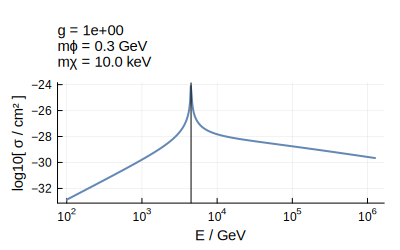
\includegraphics[width=8cm]{images/sf_xsec_1}}
    \caption{The Scalar-Fermion cross-section as a function of energy, for fixed model parameters. As expected, the scale of the cross-section is roughly equal to that of neutrino DIS scattering at 1 TeV, $\sim 10^{-30} \frac{1}{\text{cm}^2}$.}
\end{figure}

\begin{figure}[h!]
    \raisebox{-3.4cm}{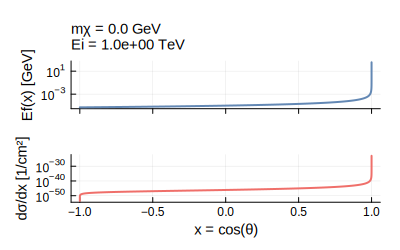
\includegraphics[width=16cm]{images/sf_diffxsec_dcostheta}}
    \caption{The cross-section is highly forward peaked. As expected, the scale of the cross-section at its peak is roughly equal to  $\sim 10^{-30} \frac{1}{\text{cm}^2}$.}
\end{figure}

\begin{figure}[h!]
    \raisebox{-3.4cm}{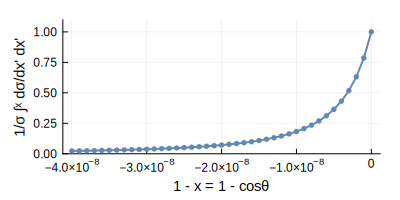
\includegraphics[width=16cm]{images/sf_costheta_CDF}}
    \caption{Partial integrals of $\frac{d\sigma}{d\cos\theta}$, in the region very close to $\cos\theta = 1$.}
\end{figure}

\end{document}  